\section{Detector Calibration}

%Section goals:
%\begin{itemize}
%\item Discussion of unique calibration challenges in \nuprismlite (Hiro's workshop talk) \red{(HT)}
%\begin{itemize}
%\item moving detector
%\item deployment of sources in the ID
%\end{itemize}
%\end{itemize}

The calibration systems for \nuprismlite will largely borrow from the existing Super-K calibration systems. However, \nuprismlite will also face some unique challenges:
\begin{itemize}
\item The PMT frame will move within the water volume.
\item Accessing the inner detector is more difficult when the position of the top of the detector is not fixed.
\end{itemize}
To address these issues, \nuprismlite will consist of calibration sources that are fixed within the ID (e.g. laser balls, LEDs, and scintillation cubes), as well as sources that can be lowered though remote-controlled access portals (e.g. radioactive sources). It is expected that each time the detector is moved, all of the PMTs will need to be recalibrated. This can be accomplished using the fixed light sources within the ID, and additional calibration runs with radioactive sources will be taken for each new detector position.

In addition to the detector response, it will also be necessary to precisely determine both the relative position of the PMTs within the ID, as well as the absolute position of the PMT frame within the water volume. This will be accomplished with a laser calibration system. An R\&D program is planned to demonstrate the effectiveness of such a system when operated in water.

As \nuprism will essentially reuse many of the established Super-K calibration techniques, the remainder of this section will provide a brief description of Super-K calibration systems. Further details can be found elsewhere~\cite{Fukuda:2002uc, SK_calib_paper}.

\subsection{Overview of Super-K Calibration Systems}

%Section goals:
%\begin{itemize}
%\item Description of relevant SK detector systems -- Hide's talk at the collaboration meeting  \red{(HKT)}
%\end{itemize}

This section overviews Super-K detector calibrations.
For further details, reader can also refer to \cite{Fukuda:2002uc, SK_calib_paper}.

The Super-K detector calibration can be divided into two steps;
the detector hardware calibrations and the calibrations for physics analyses.
The first step is common over all physics analyses, but the second step is
designed for each physics analysis goal.

\subsubsection{Detector hardware calibrations}

The detector hardware calibrations (measurements) consist of several parts:
\begin{itemize}
  \item Geometrical surveys: tank geometry, PMT positions
  \item Geomagnetic field
  \item PMT calibration: gain, photo-detection efficiency
  \item Readout channel (PMT and electronics) calibrations: linearity, timing, timing resolution
  \item Optical properties: water, PMT glass, black sheet, etc (for detector MC tuning)
  \item Water temperature
\end{itemize}
All of these calibrations and measurements are indispensable to understand the detector and
to model the detector in the simulation.
%
This section focuses on the PMT calibrations and readout channel calibrations, which
will be most relevant to \nuprismlite.

The PMT calibration procedure can be divided into three large steps;
1) pre-calibration, 2) post-installation calibration, 3) detector monitoring.
At the stage of `pre-calibration', a fraction of all Super-K PMTs have been
calibrated prior to the installation, e.g. a tuning of PMT gain.
The pre-calibrated PMT, called {\it standard PMTs}, were used to calibrate all
other PMTs {\it in-situ} after installed, at the stage of post-installation calibration.
Once all PMT are calibrated, the stability of the PMTs is monitored continuously
for the lifetime of the experiment.
%
The following sections discuss our ideas for each of the PMT
calibration steps.

\paragraph{Pre-calibration}

SK has 420 standard PMTs, which corresponds to about 4\% of all SK PMTs.
The SK standard PMTs were calibrated prior to the installation by adjusting
HV values to have identical charge ($\sim30$ p.e.) over the standard PMTs.
For the pre-calibration, SK employed a xenon lamp and scintillator ball.
Figure~\ref{fig:sk_precalib_setup} shows a schematic diagram of the pre-calibration
set-up.
\begin{figure}[htb]
  \centering
  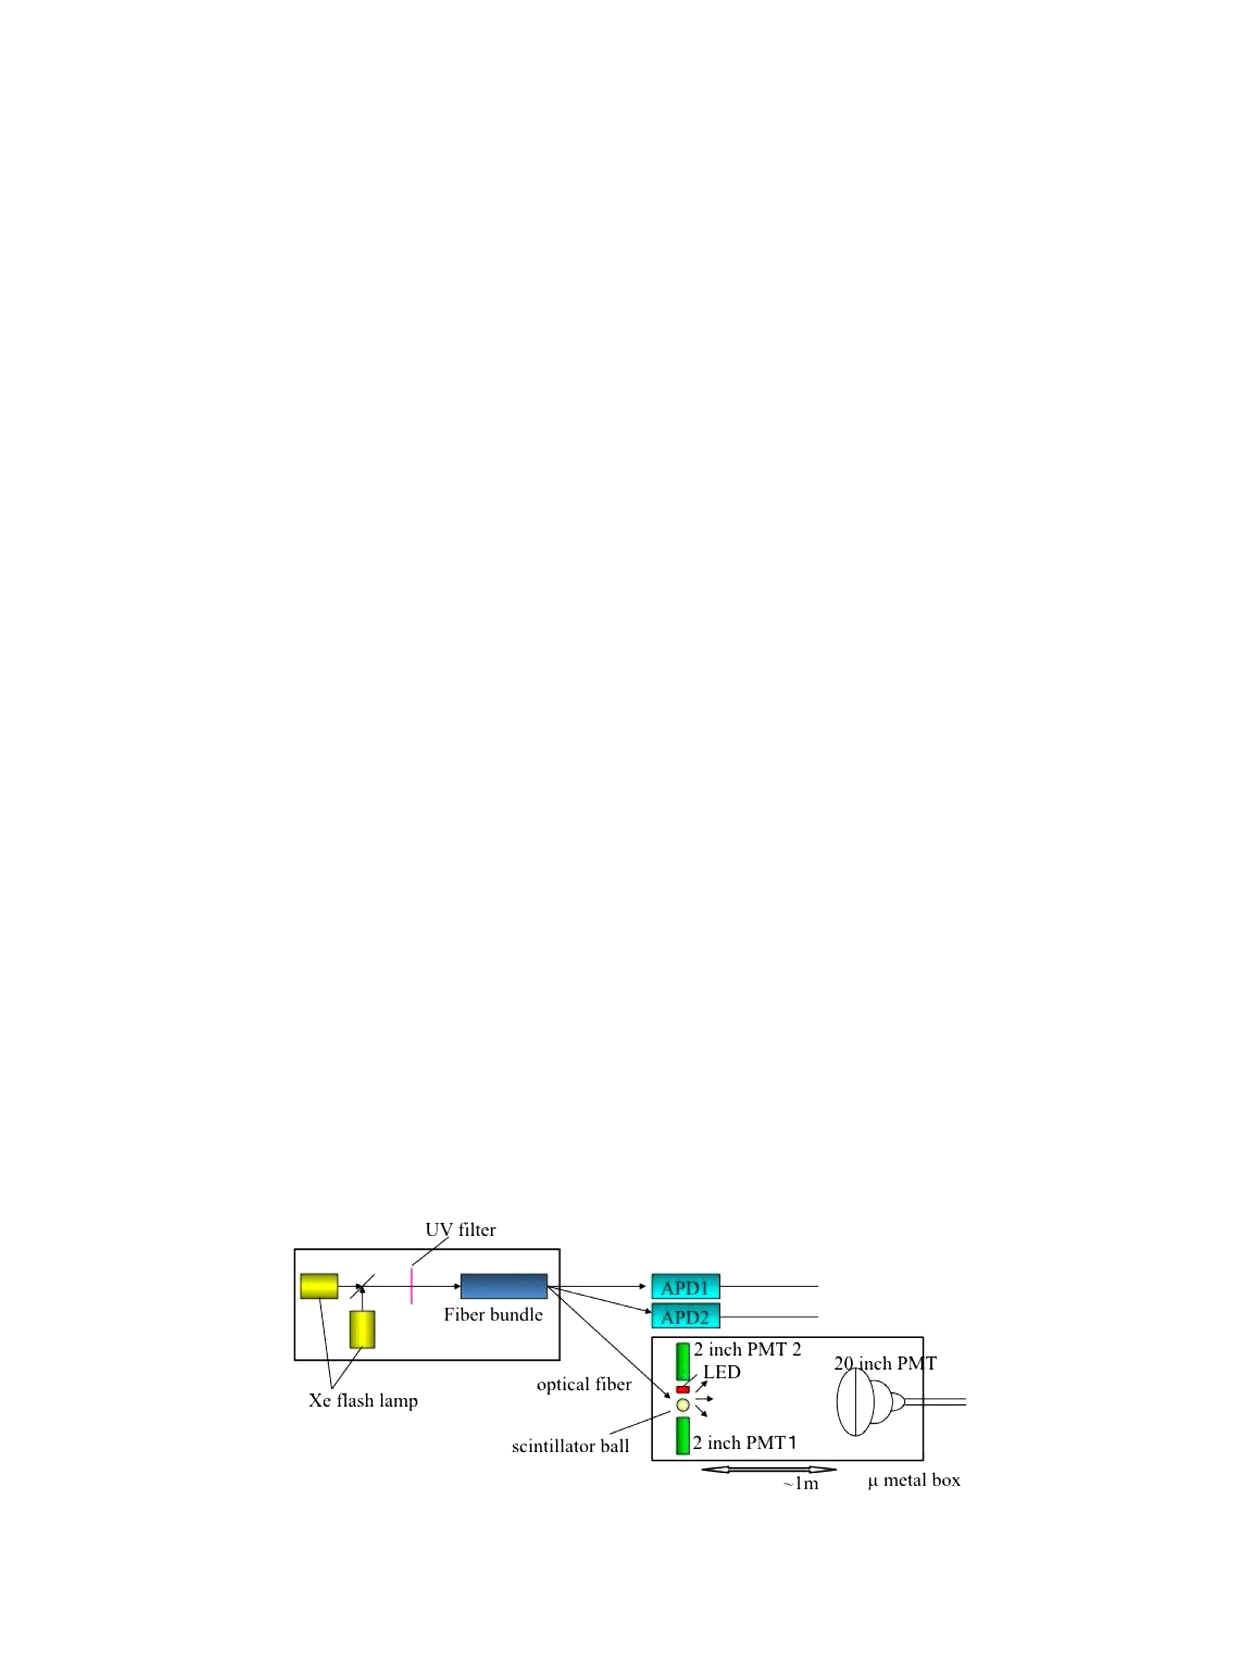
\includegraphics[width=9cm]{figures/sk_precalib_setup.pdf}
  \caption{SK pre-calibration set-up. (Figure quoted from \cite{SK_calib_paper})}
  \label{fig:sk_precalib_setup}
\end{figure}

The SK standard PMTs were installed in the tank in a geometrically symmetric configuration.
Figure~\ref{fig:sk_precalib_PMT_layout} shows the location of the standard PMTs
in SK inner detector.
\begin{figure}[htb]
  \centering
  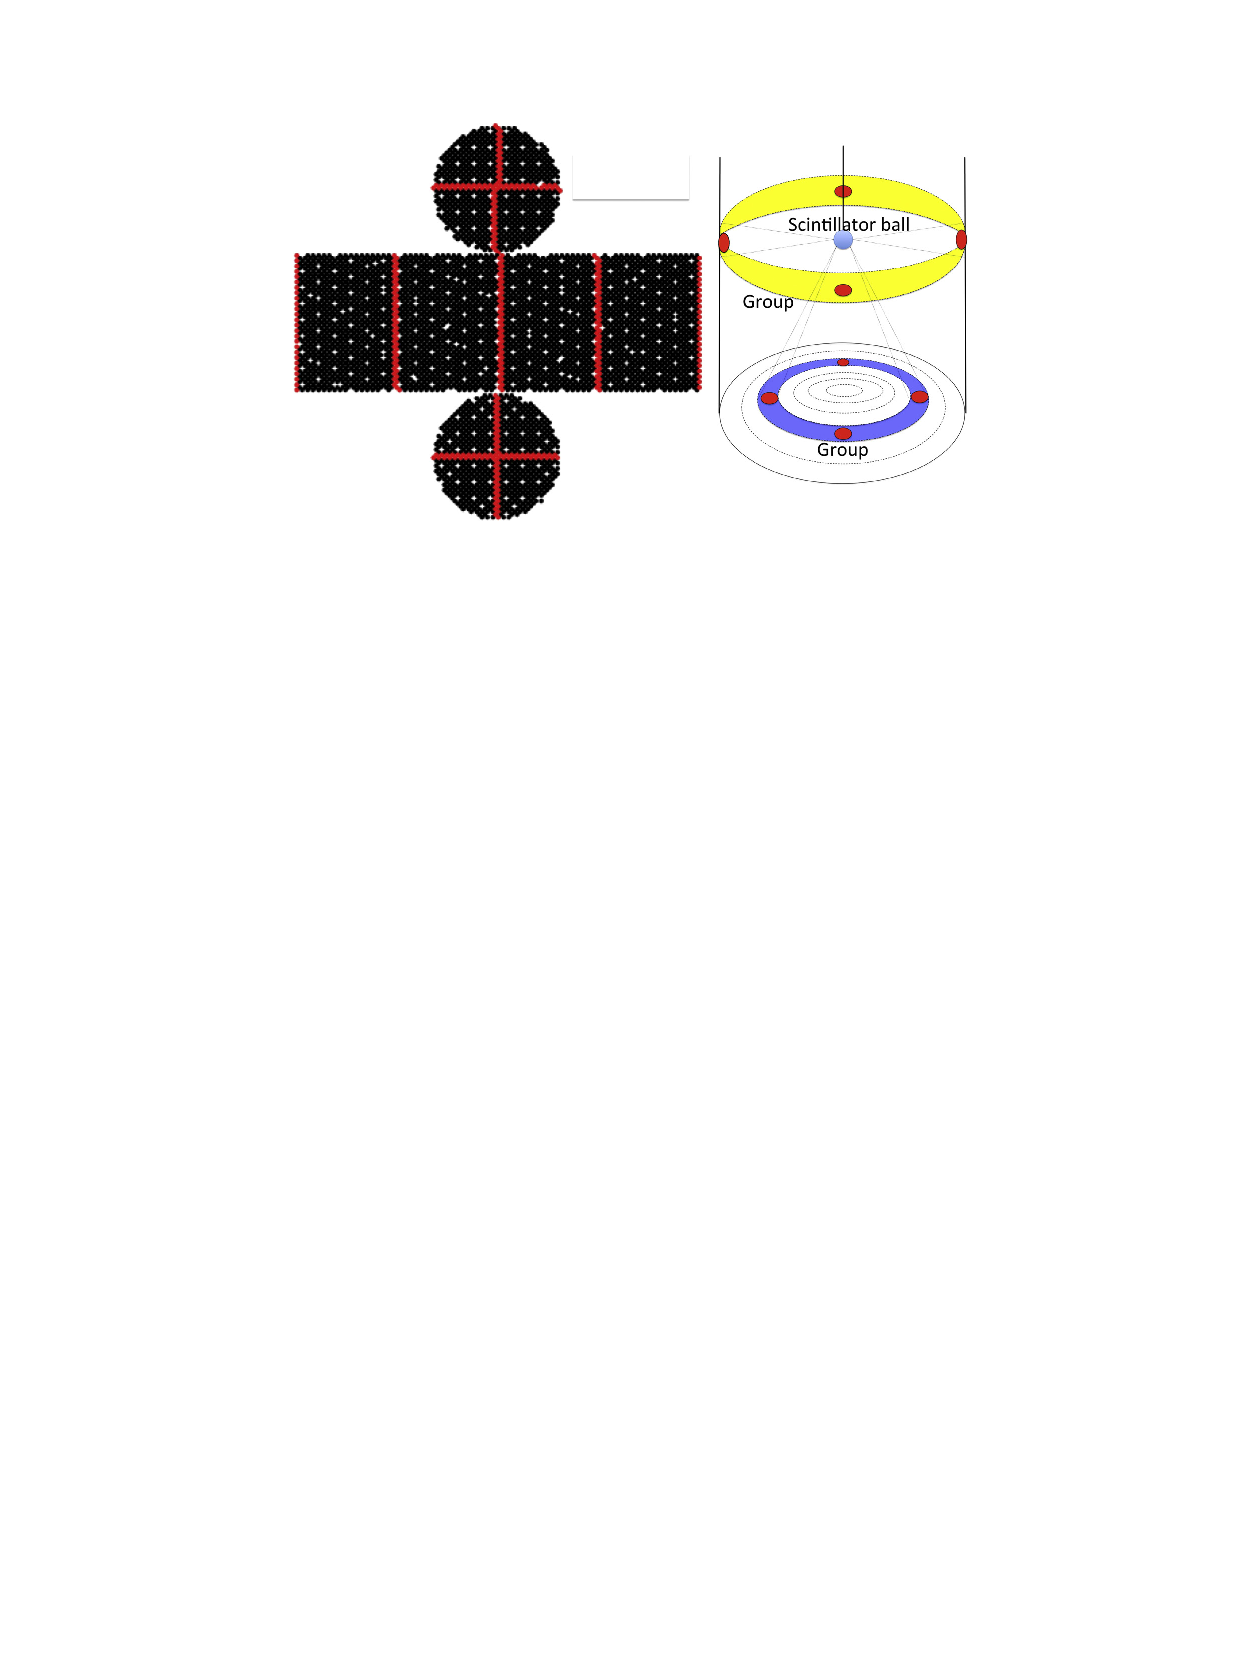
\includegraphics[width=9cm]{figures/sk_precalib_PMT_layout.pdf}
  \caption{Layout of SK standard PMTs. (Figure quoted from \cite{SK_calib_paper})}
  \label{fig:sk_precalib_PMT_layout}
\end{figure}
%In SK pre-calibration, HV values of the standard PMTs were determined to obtain
%the same pulse height (30 p.e.) between them.

\paragraph{Post-installation calibrations}

In the post-installation calibration, all PMTs other than the standard PMTs
were calibrated {\it in-situ} after installed.
%
At this stage, all PMT parameters were determined and measured.
We will discuss the following items in this section,
\begin{itemize}
% --------------------------
\item HV (gain) tuning\\
  Tune HV for all PMTs, referencing to the standard PMTs by using the Xe lamp and deploying
  a scintillator ball in the tank (the same light source used in the pre-calibration).
  Move the scintillator ball along Z-axis (height direction), and tune HV group-by-group,
  where the group is defined by Fig.~\ref{fig:sk_precalib_PMT_layout}.

% --------------------------
\item Charge to photo-electron conversion\\
  Conversion factor of charge (pC) to photo-electron (p.e.) were obtained by measuring 1~p.e.
  distribution.
  SK deployed ``nickel source'' in the tank, that generate 1~p.e. level of light, where the
  nickel source is nickel-californium source; Ni(n,$\gamma$)Ni, E$_{\gamma}\sim$9~MeV.
  %Figure~\ref{fig:sk_1pe_dist} shows 1~p.e. distribution of SK.
  %\begin{figure}[htb]
  %  \centering
  %  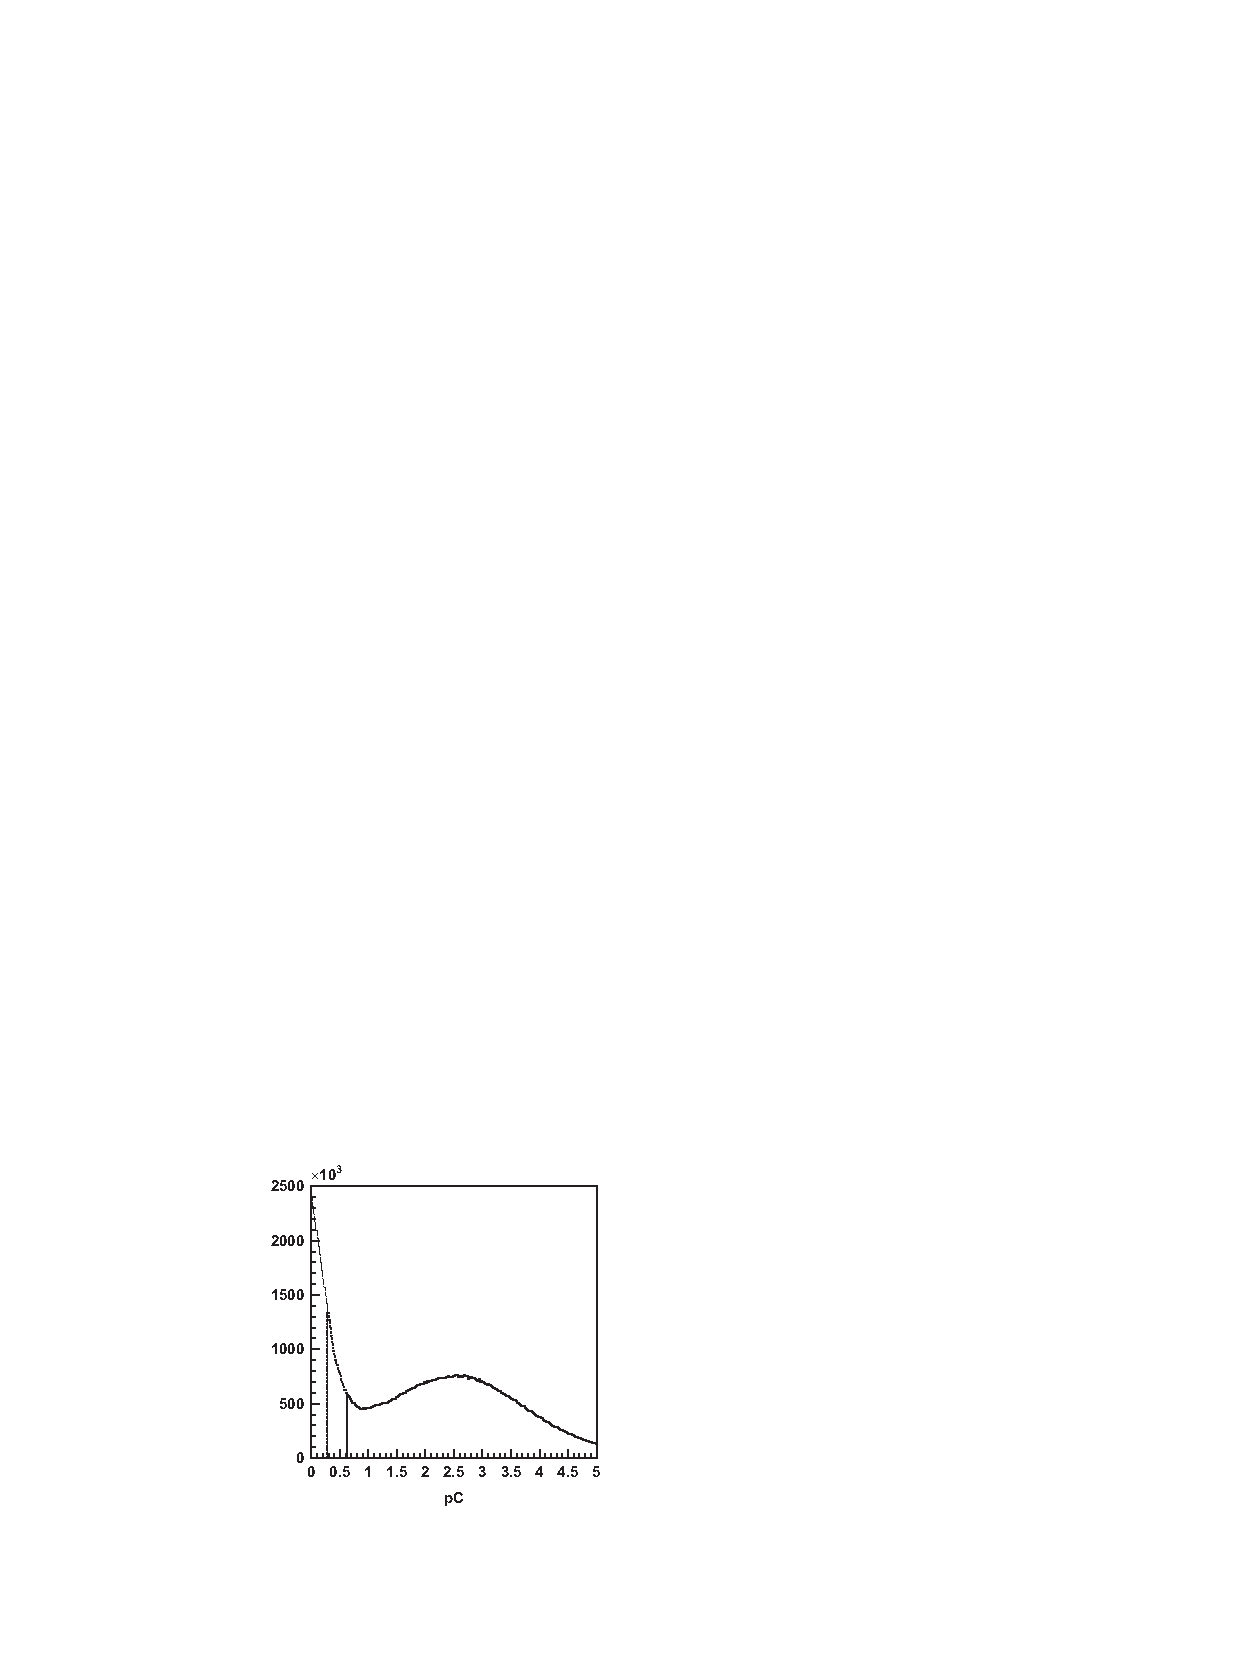
\includegraphics[width=0.3\textwidth]{sk_1pe_dist.pdf}
  %  \caption{SK 1~p.e. distribution. Note that this distribution is accumulated over all PMTs.
  %    (Figure quoted from \cite{SK_calib_paper})}
  %  \label{fig:sk_1pe_dist}
  %\end{figure}
  Figure~\ref{fig:sk_nickel_source} shows the SK nickel source.
  \begin{figure}[htb]
    \centering
    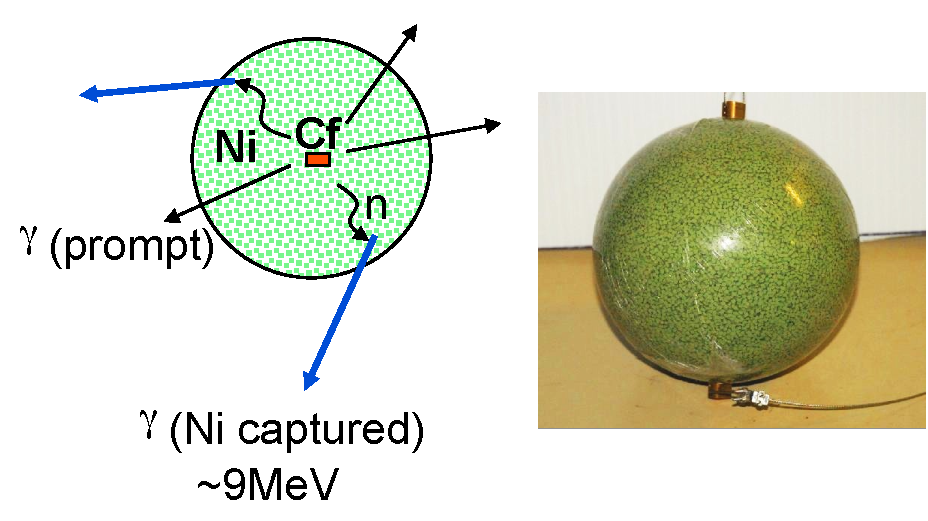
\includegraphics[width=9cm]{figures/sk_nickel_source.pdf}
    \caption{SK ``Nickel source'' (Figure quoted from \cite{SK_calib_paper})}
    \label{fig:sk_nickel_source}
  \end{figure}

% --------------------------
\item Photo-detection efficiency\\
  The photo-detection efficiency, $\epsilon$, is defined by Quantum Efficiency times Collection
  Efficiency (CE).
  Hit rate (Nhit) for 1 p.e. level of light is proportional to the photo-detection efficiency;
  $N_{hit} \propto N_{photon} \cdot \epsilon$.
  For this measurement, SK used the Nickel source to evaluate the hit rate, and compare with MC
  to evaluate {\it relative} efficiency over all PMTs.
  
% --------------------------
\item Timing calibration\\
  Calibration for time response of readout channel (PMT and electronics), e.g. {\it time-walk}
  effect.
  SK employed N$_2$-dye laser and deployed diffuser-ball in tank, that light source can generate
  0.1$\sim$1000~p.e. level light and covers the entire dynamic range of electronics.
  Evaluate TQ-maps for every single PMTs, and evaluate detector timing resolution (for MC input).

\end{itemize}


\subsubsection{Calibrations for physics analyses}

The calibrations for physics analyses need to be designed for physics goal basis.
This section describes the calibrations used for SK atmospheric neutrino and T2K
analyses, that relevant to \nuprismlite physics goals.

\paragraph{Photon yield and charge scale}

Although several detailed detector calibrations have been carried out, there are
uncertainties on the photon propagation and photon detection of the detector,
that need to be tuned in the detector simulation using a well known control samples.
For that, SK uses cosmic-ray muons, called ``vertical through-going muons''.
Figure~\ref{fig:sk_thru_muon} shows a schematic of vertical through-going muon event
of SK.
\begin{figure}[htb]
  \centering
  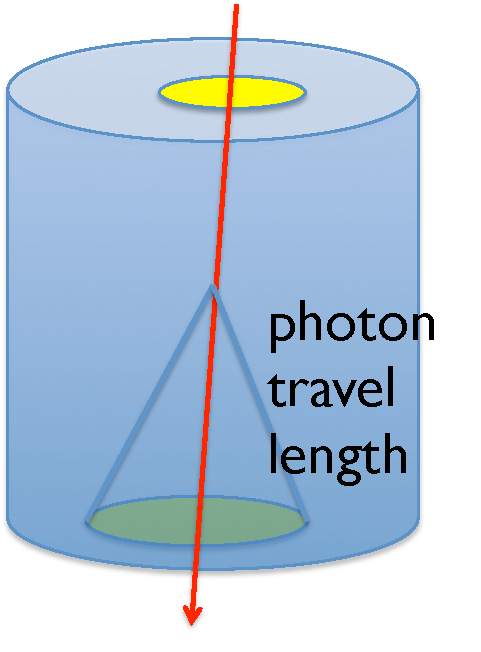
\includegraphics[height=6cm]{figures/sk_thru_muon.pdf}
  \caption{Schematic of SK vertical through-going muon events.}
  \label{fig:sk_thru_muon}
\end{figure}
The absolute photon yield and charge scale in the detector simulation have been tuned
to data using the vertical through-going muon events that provide known muon track length
and Cherenkov photon travel distance.


\paragraph{Momentum and energy scale}

SK event reconstruction algorithm uses a conversion table that translate the observed total
charge in the Cherenkov ring to the particle (muons and electrons) momentum.
The conversion table is called ``momentum table'' have been evaluated using the detector
simulation by generating particles in momentum range of 10's MeV/c to GeV/c.
%
Based on all detector calibrations and the simulation tuning, the detector and simulation
are ready to use for physics analyses.
Absolute energy scale is checked using natural sources; decay electron, $\pi^{0}$ mass,
sub-GeV stopping muons, and multi-GeV stopping muons, these sources cover the energy range of
10's MeV to 10~GeV.
SK detector simulation reproduces data within $\sim2$\% and that have been continuously
monitored.
SK defines the energy scale uncertainty as the data-MC difference.
If the simulation does not reproduce the data reasonably well, the detector calibrations
and simulation tuning need to be revised.


%\subsection{Additional Calibration Systems \red{(R. Tacik \& K. Mahn)}}
%
%Section goals:
%\begin{itemize}
%\item Discussion of possible additional calibration systems to be used in \nuprismlite \red{(RT)}
%\item MiniBooNE cubes? \red{(RT)}
%\item LEDs? \red{(RT or Asher?)}
%\item ...
%\item PMT position calibration \red{(KM)}
%\end{itemize}

